\documentclass{beamer}
\usetheme{hfut}
\usepackage{xeCJK}
\usepackage{graphicx}
\usepackage{booktabs}
\usepackage{array}
\usepackage{tikz}
\setCJKmainfont{SimSun}
\setCJKmonofont{SimSun}
\makeatletter
\providecommand\Hy@PageAnchorSlide{}
\makeatother
\graphicspath{{../assets/}{./}}

\title{智学工坊：个性化学习资源生成与学习多智能体系统}
\author{中国软件杯 A3 赛题参赛作品}
\institute{合肥工业大学}
\date{2026}

\begin{document}

\begin{frame}
  \maketitle
\end{frame}

\section{项目价值}

\begin{frame}{赛题目标与产品定位}
\begin{itemize}
  \item 面向高校课程学习，解决资源繁杂、学习节奏差异和个性化辅导不足的问题。
  \item 以课程为中心组织学生画像、资料、资源生成、路径规划、答疑和评估。
  \item 使用科大讯飞星火 API 驱动正式生成能力，结合 RAG 和多智能体协作提升可靠性。
  \item 学生端关注学习闭环，教师端关注资源审核、发布质检和学情证据。
\end{itemize}
\end{frame}

\begin{frame}{核心用户与场景}
\begin{columns}
\column{0.48\textwidth}
\textbf{学生端}
\begin{itemize}
  \item 对话式构建学习画像
  \item 上传资料生成个性化资源
  \item 在课程空间获得 AI 辅导
  \item 根据路径完成学习闭环
\end{itemize}
\column{0.48\textwidth}
\textbf{教师端}
\begin{itemize}
  \item 上传课程资料建设课程
  \item 审核 AI 生成资源
  \item 进行发布前质量检查
  \item 查看班级画像和学习证据
\end{itemize}
\end{columns}
\end{frame}

\section{系统架构}

\begin{frame}{总体架构}
\begin{center}
\begin{tikzpicture}[node distance=1.2cm, every node/.style={font=\small}]
\node[draw, rounded corners, fill=cyan!10, minimum width=8.5cm, minimum height=0.8cm] (ui) {Vue 3 前端：学生工作区 / 教师工作台 / 课程空间};
\node[draw, rounded corners, fill=green!10, below of=ui, minimum width=8.5cm, minimum height=0.8cm] (api) {Spring Boot 后端：课程、画像、任务、审核、学习事件};
\node[draw, rounded corners, fill=orange!10, below of=api, minimum width=8.5cm, minimum height=0.8cm] (agent) {Python 多智能体服务：RAG、LangGraph、讯飞星火、内容审计};
\node[draw, rounded corners, fill=gray!10, below of=agent, minimum width=8.5cm, minimum height=0.8cm] (data) {课程资料 / 上传文档 / 学习记录 / 模型调用证据};
\draw[->, thick] (ui) -- (api);
\draw[->, thick] (api) -- (agent);
\draw[->, thick] (agent) -- (data);
\draw[->, thick] (data.east) .. controls +(2,0) and +(2,0) .. (api.east);
\end{tikzpicture}
\end{center}
\end{frame}

\begin{frame}{多智能体协同链路}
\begin{enumerate}
  \item 画像抽取：从对话、测评和学习事件中抽取 8 个维度学生特征。
  \item 知识诊断：识别课程知识短板、先修缺口和易错点。
  \item 路径规划：生成动态学习步骤和资源推送顺序。
  \item 资源生成：协作产出讲义、题库、思维导图、拓展阅读、代码实操、视频脚本、PPT 共 7 类资源。
  \item 智能辅导：RAG 限定课程资料答疑，输出文字 + Mermaid 图解。
  \item 班级分析：识别班级薄弱点、风险学生并给出干预建议。
  \item 内容审计：检查引用覆盖、事实性断言、敏感内容和发布门禁。
\end{enumerate}
\centering\footnotesize（十余个角色智能体由 LangGraph 编排，后端统一调度，全链路可追踪）
\end{frame}

\section{产品设计}

\begin{frame}{学生端：我的课程}
\begin{figure}
\centering
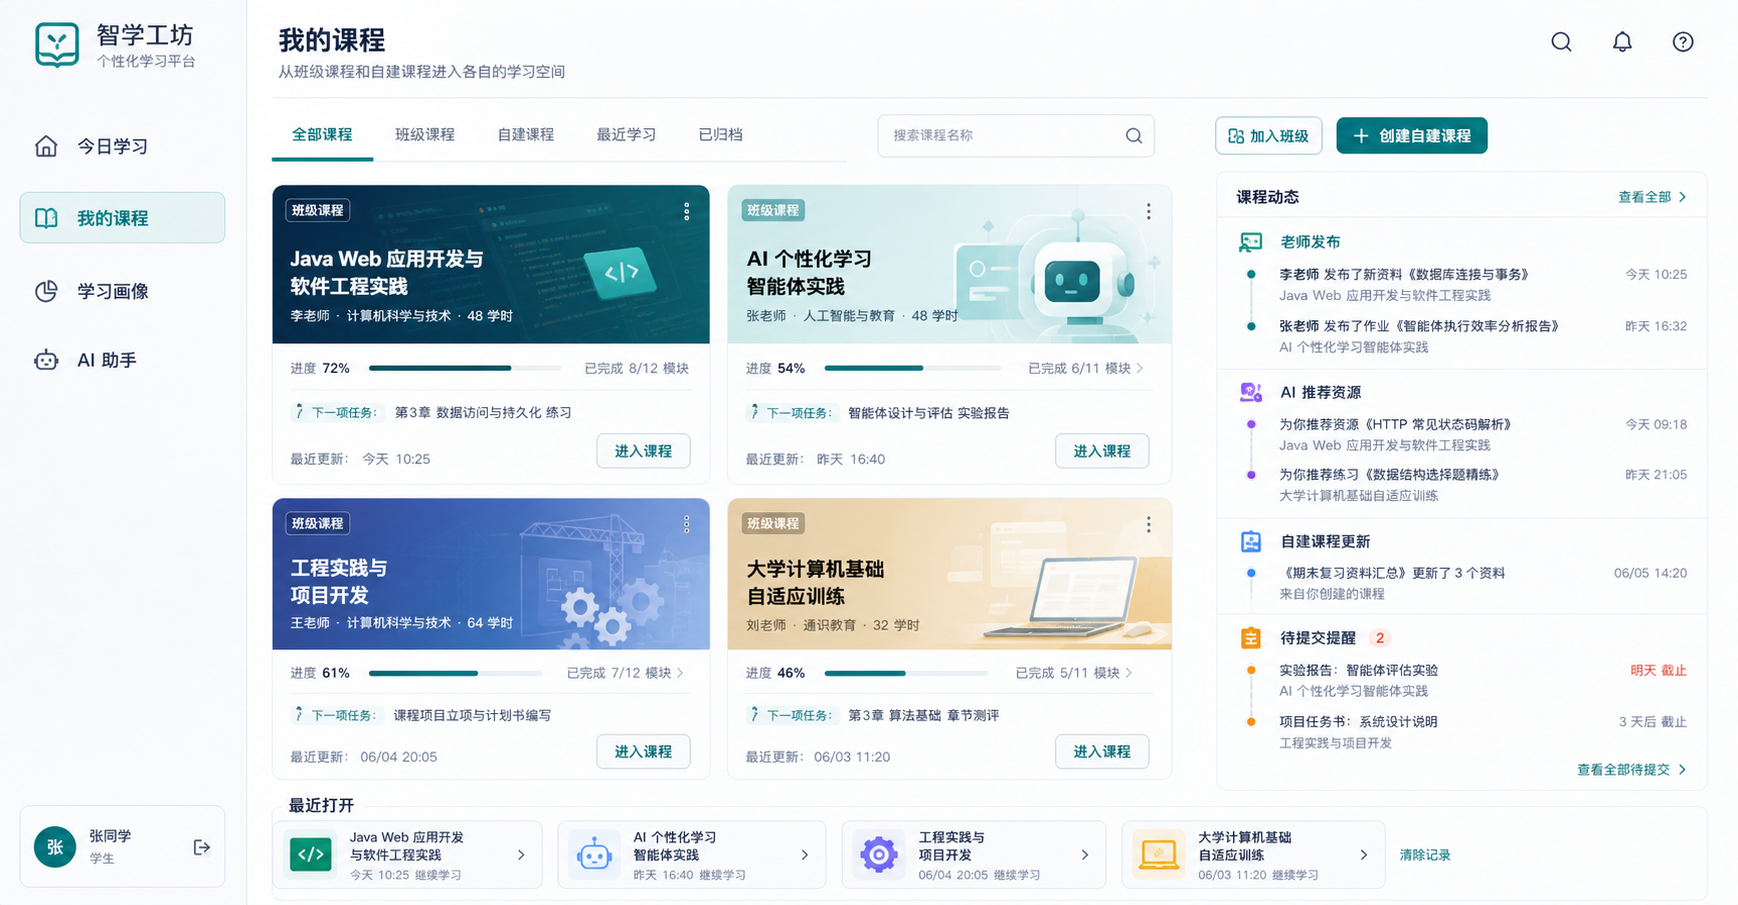
\includegraphics[width=0.92\textwidth]{01-my-courses-target.png}
\end{figure}
\end{frame}

\begin{frame}{课程详情：课程内学习闭环}
\begin{figure}
\centering
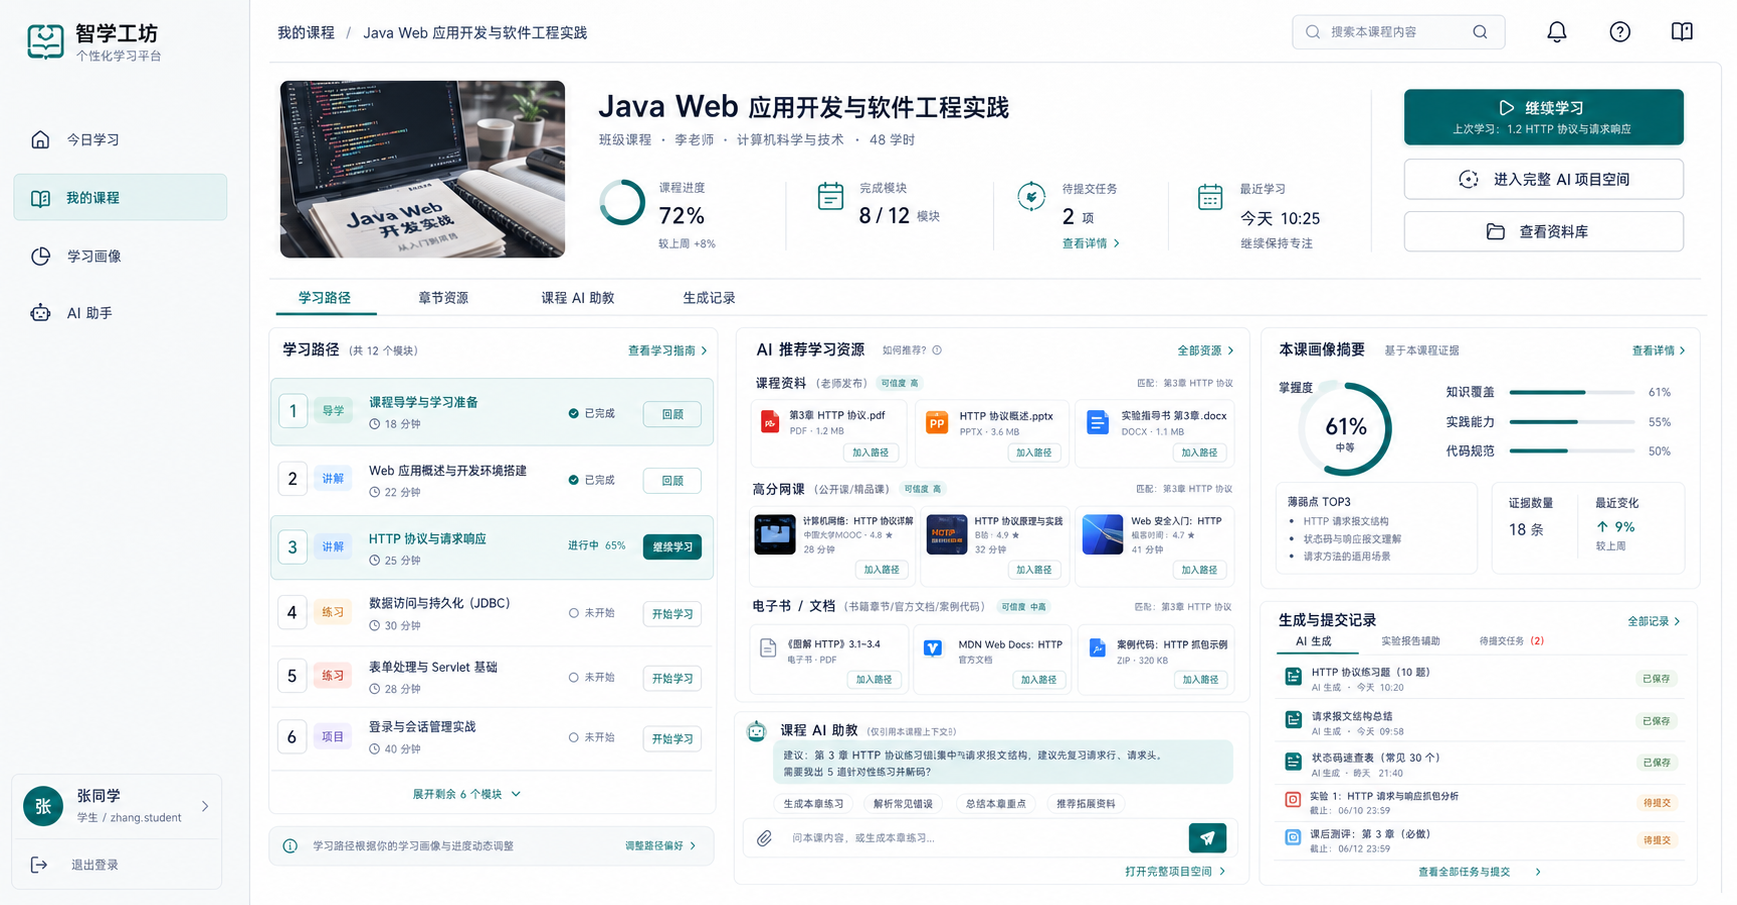
\includegraphics[width=0.92\textwidth]{04-course-detail-target.png}
\end{figure}
\end{frame}

\begin{frame}{AI 助手：课程项目空间}
\begin{figure}
\centering
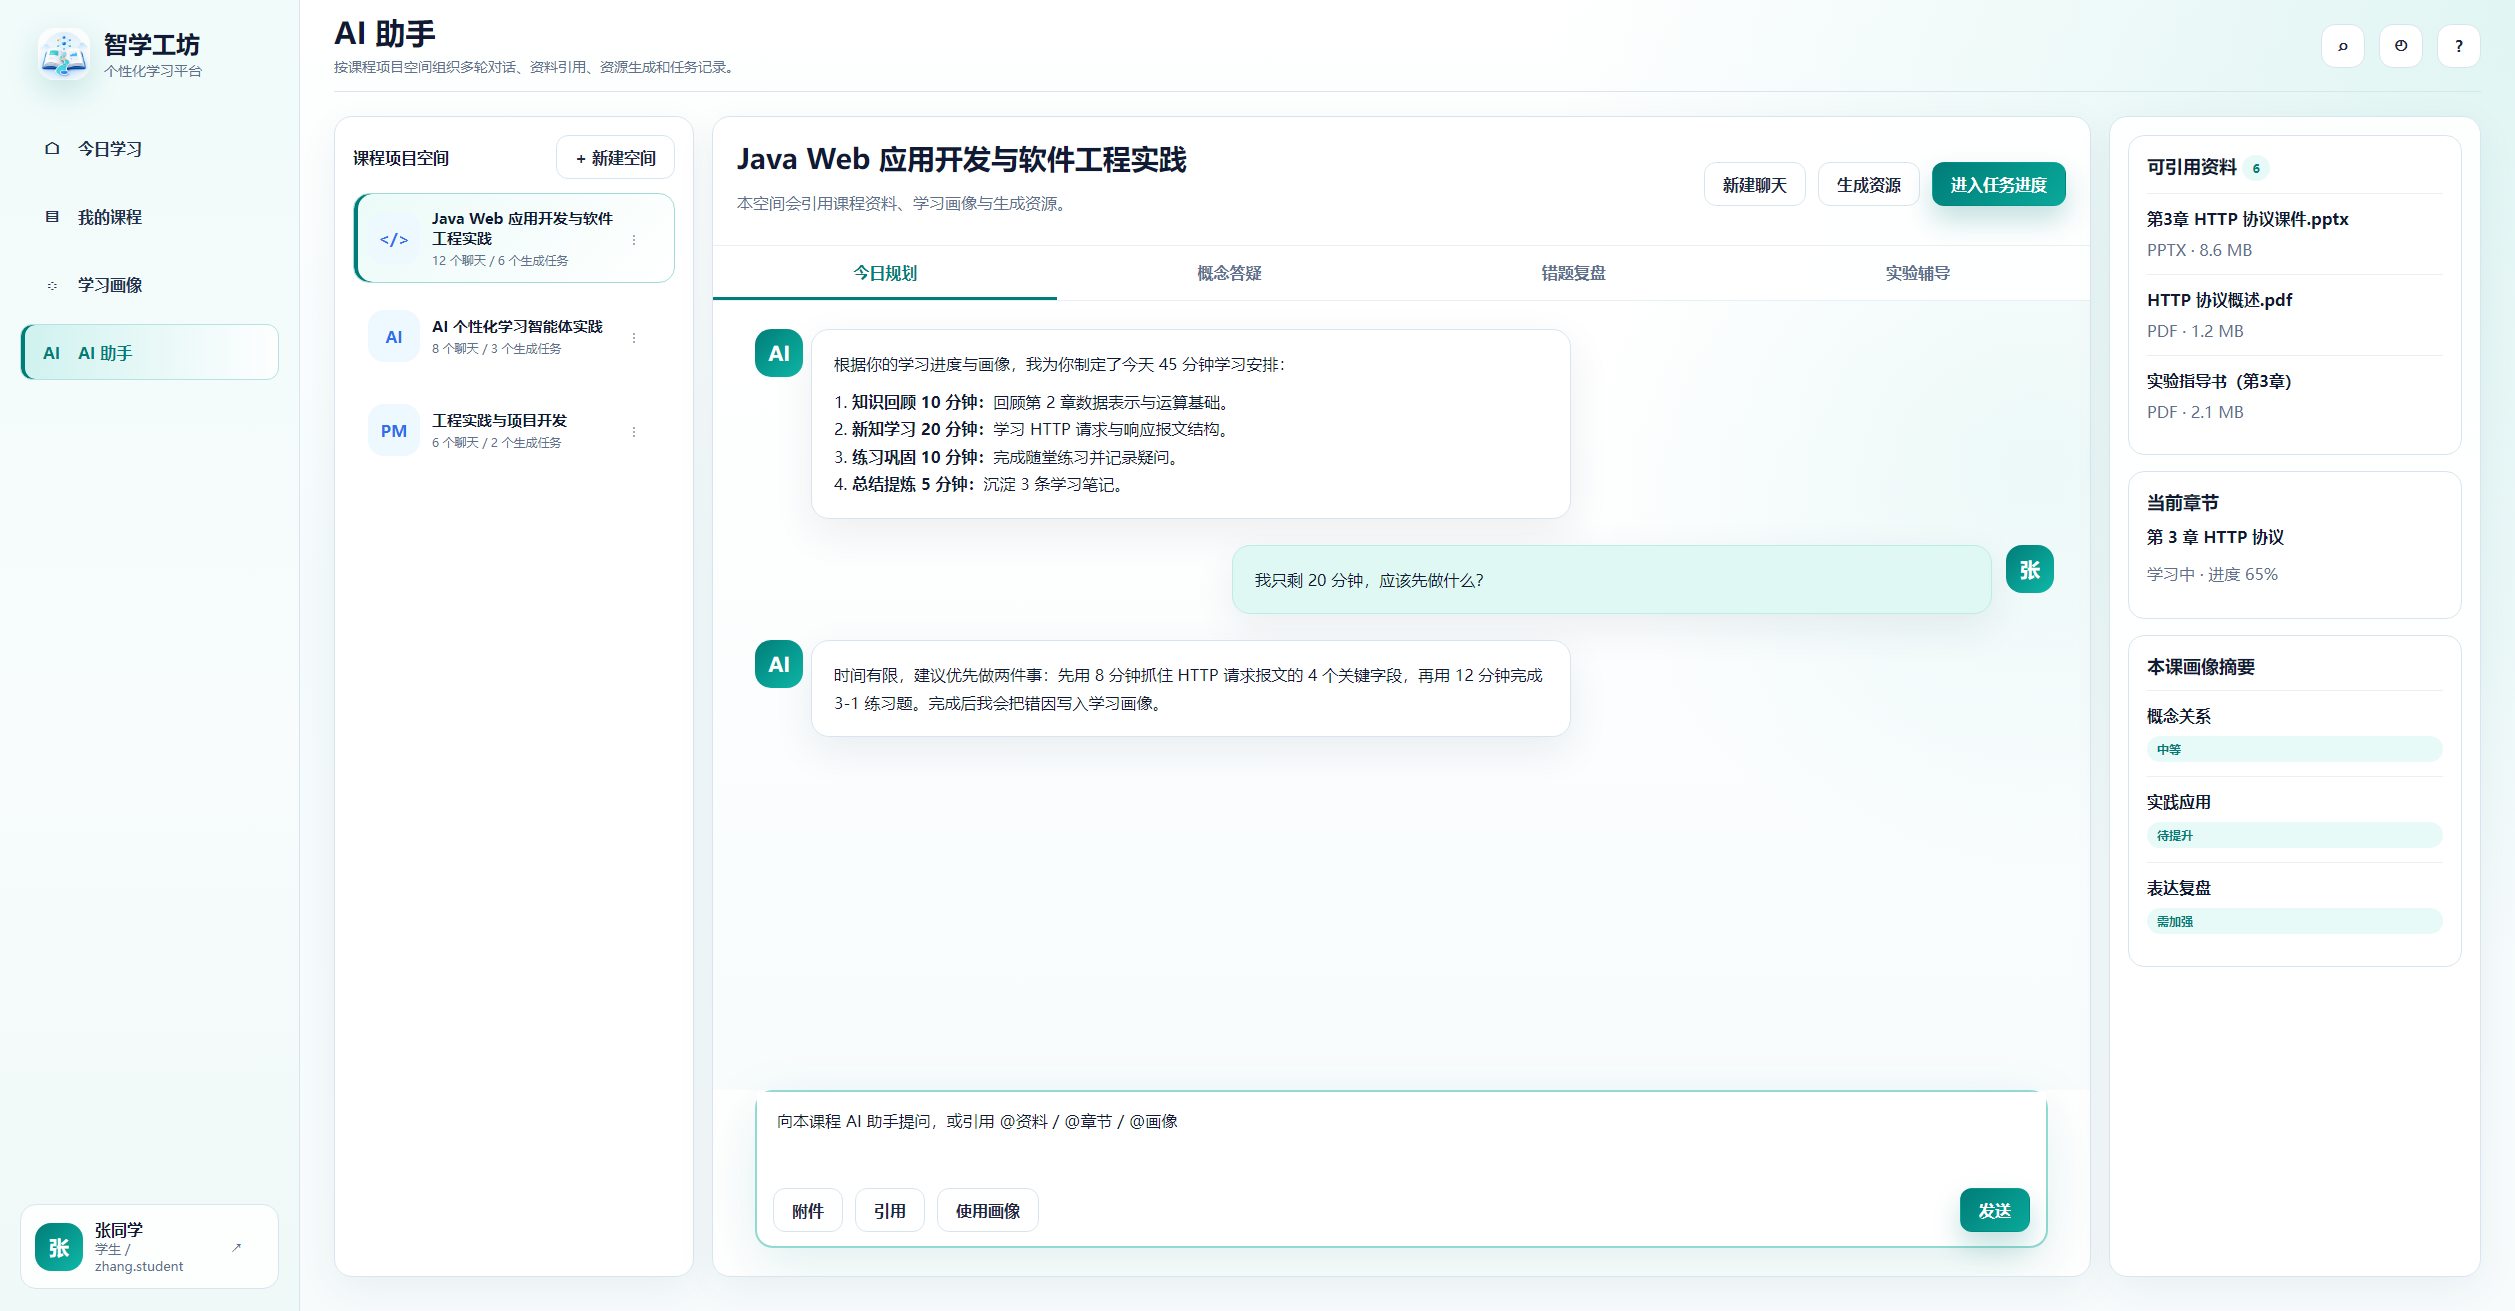
\includegraphics[width=0.92\textwidth]{01-ai-assistant-v2.png}
\end{figure}
\end{frame}

\begin{frame}{学习画像：跨课程综合评估}
\begin{figure}
\centering
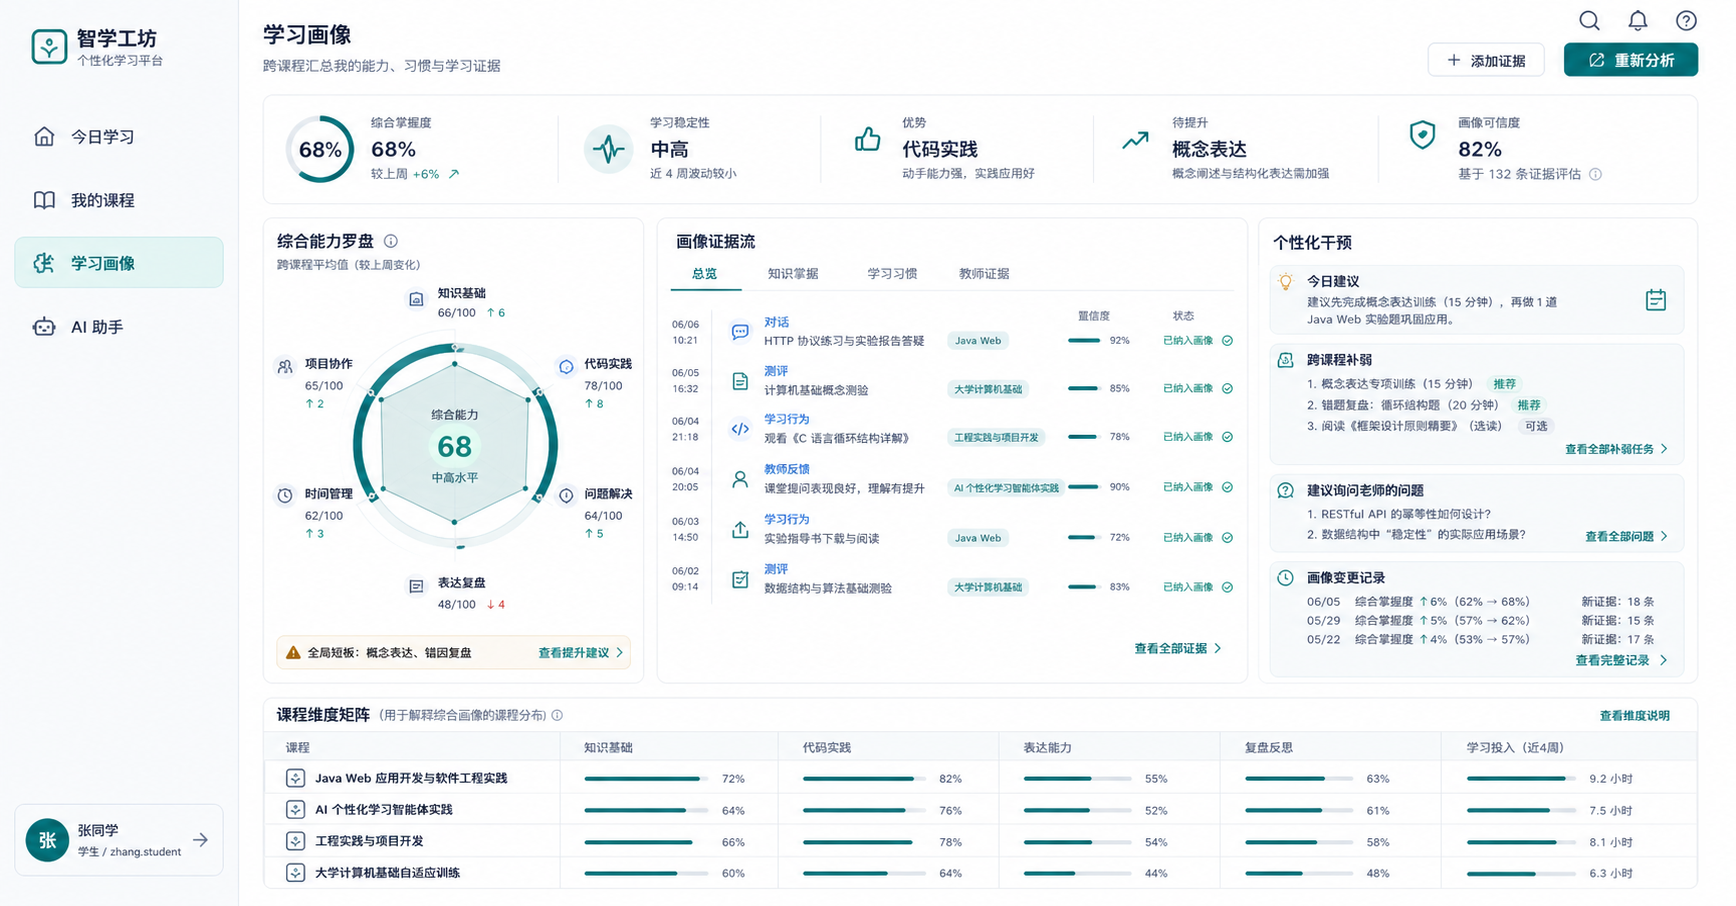
\includegraphics[width=0.92\textwidth]{03-learning-profile-target.png}
\end{figure}
\end{frame}

\begin{frame}{教师端：教学工作台}
\begin{figure}
\centering
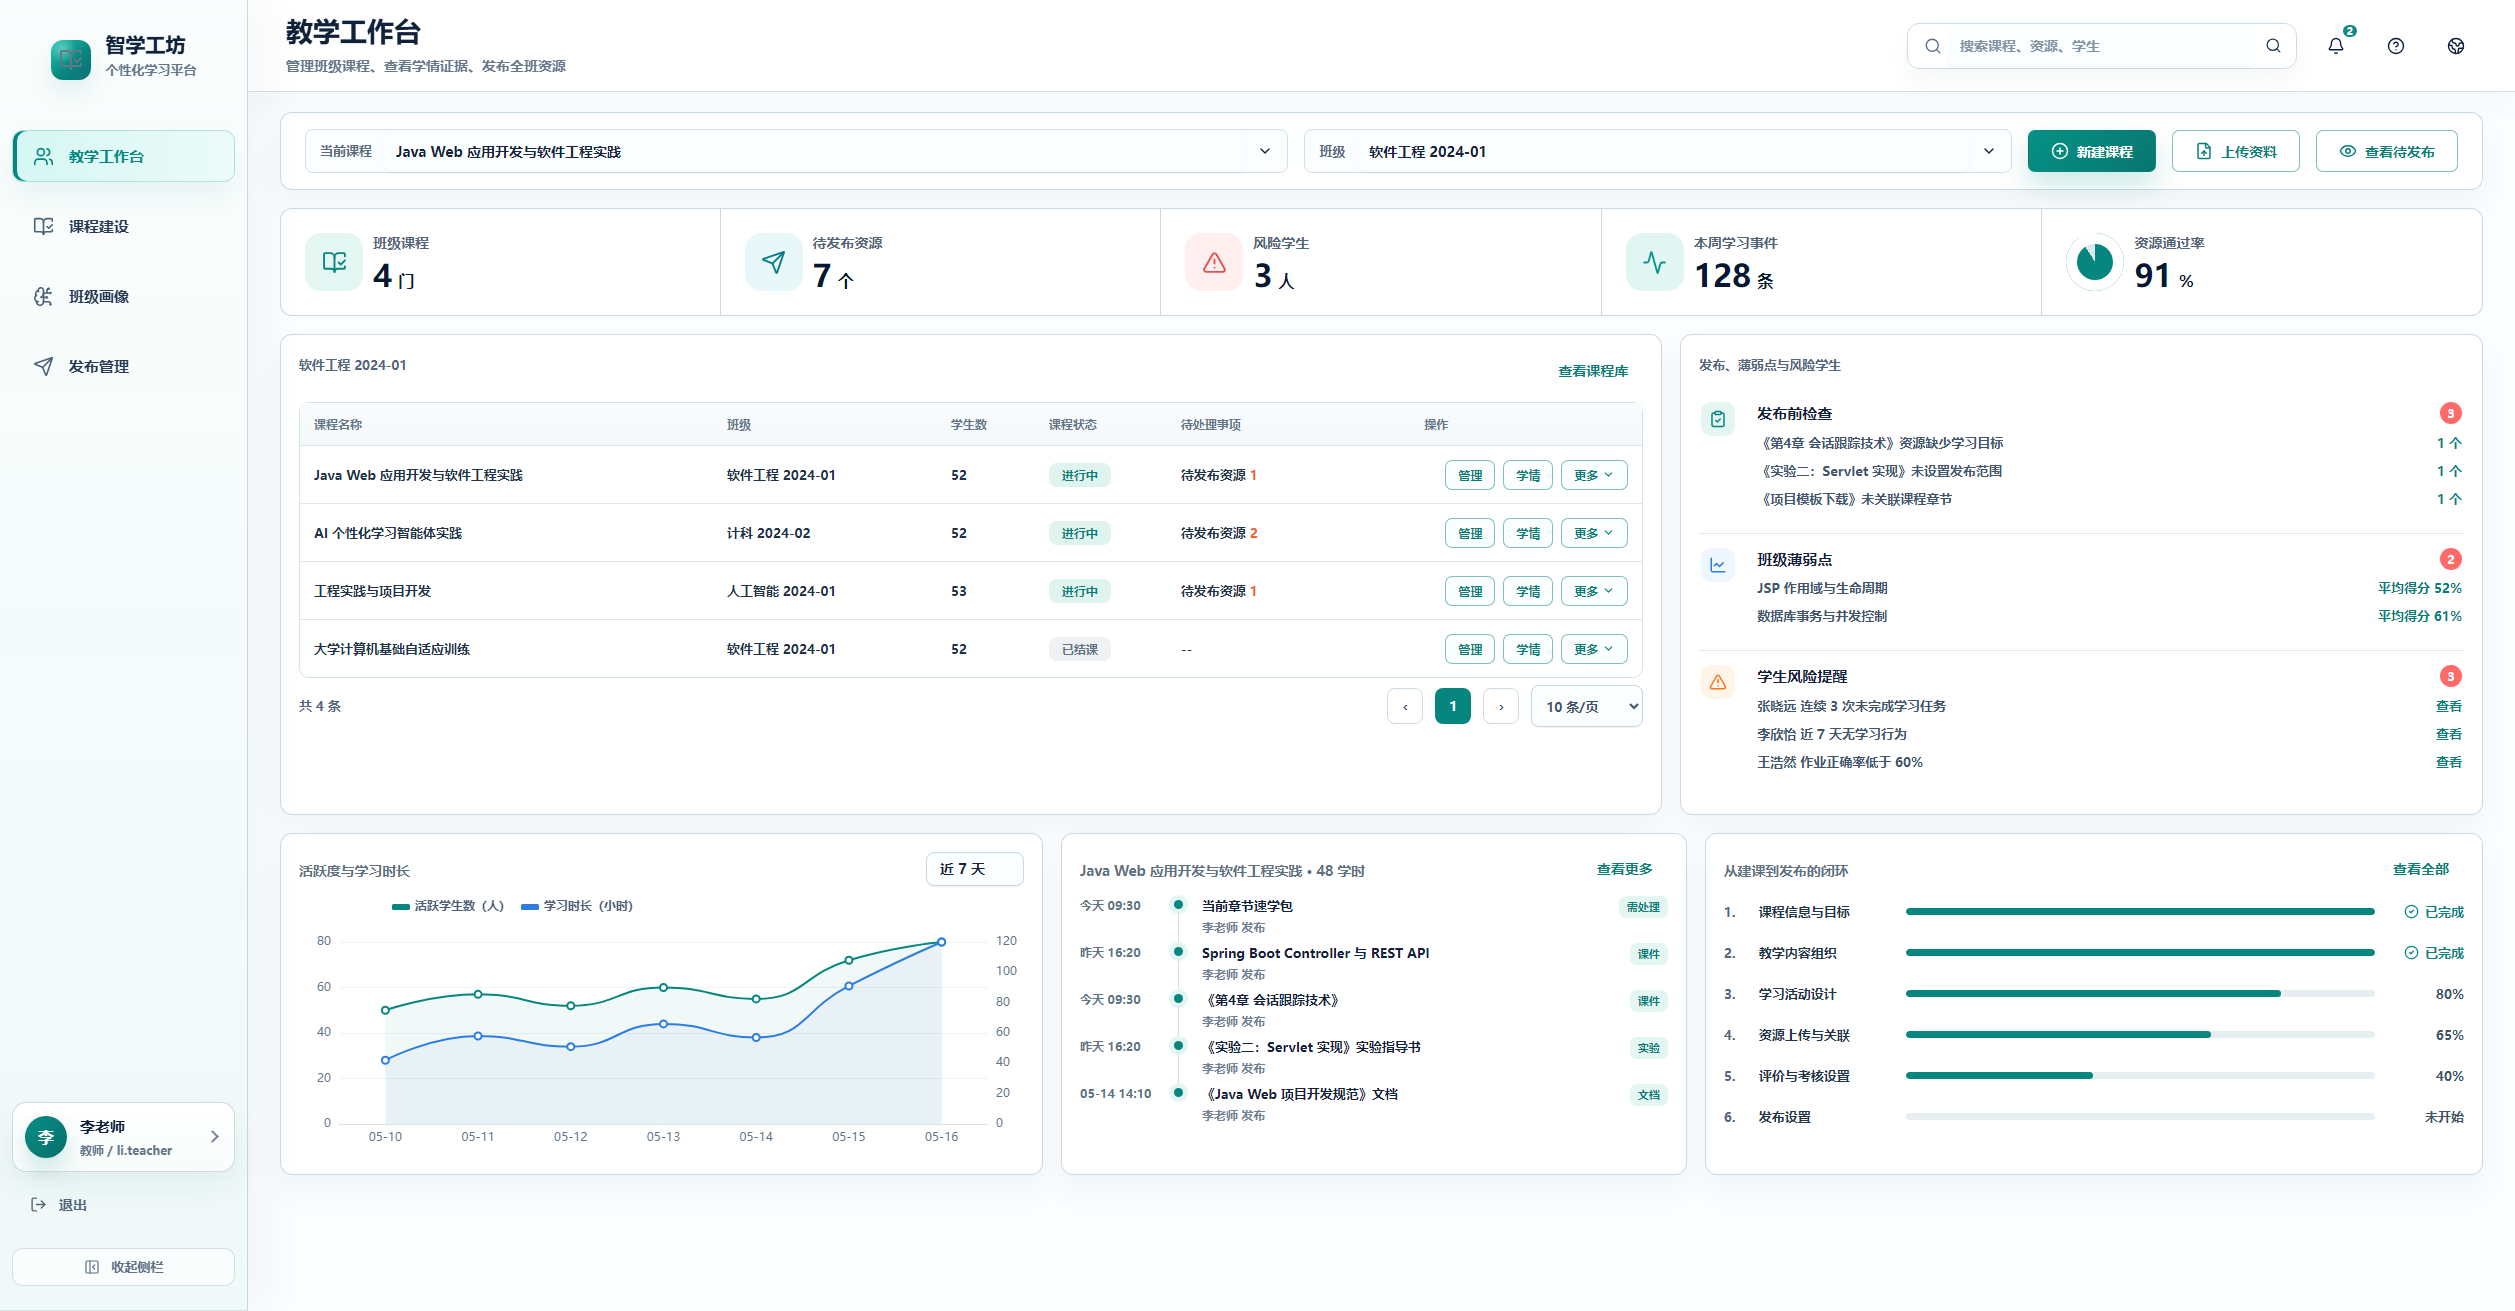
\includegraphics[width=0.92\textwidth]{teacher-workbench-approved.png}
\end{figure}
\end{frame}

\begin{frame}{教师端：课程建设}
\begin{figure}
\centering
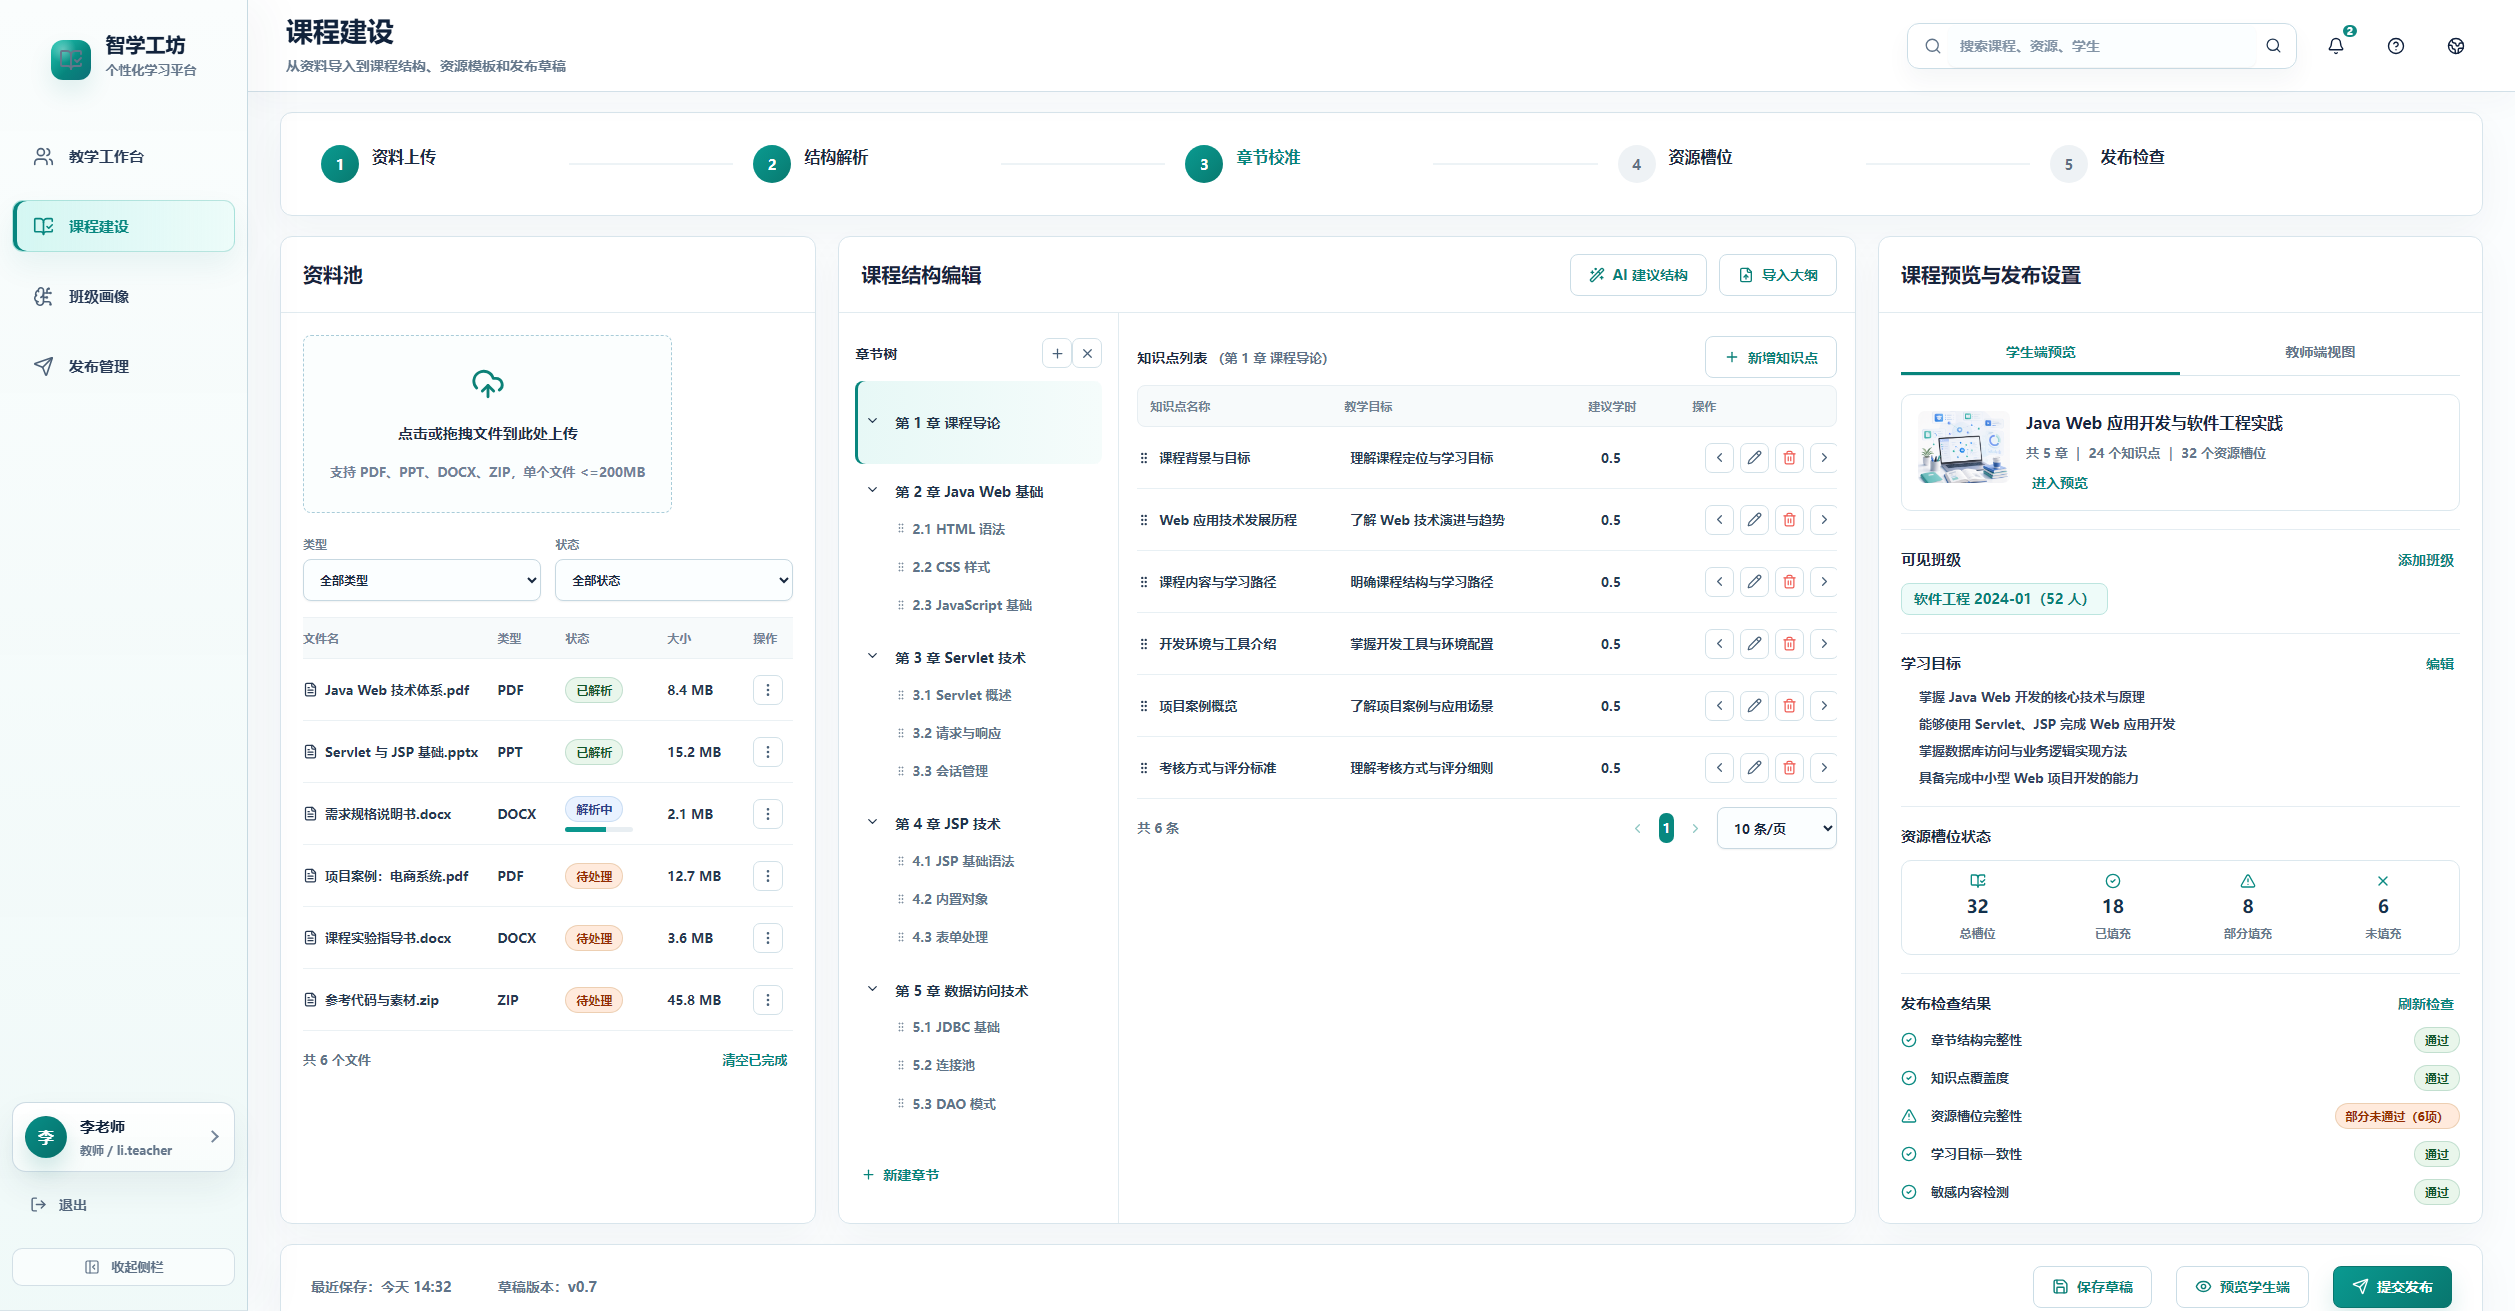
\includegraphics[width=0.92\textwidth]{teacher-course-builder-approved.png}
\end{figure}
\end{frame}

\begin{frame}{教师端：班级画像}
\begin{figure}
\centering
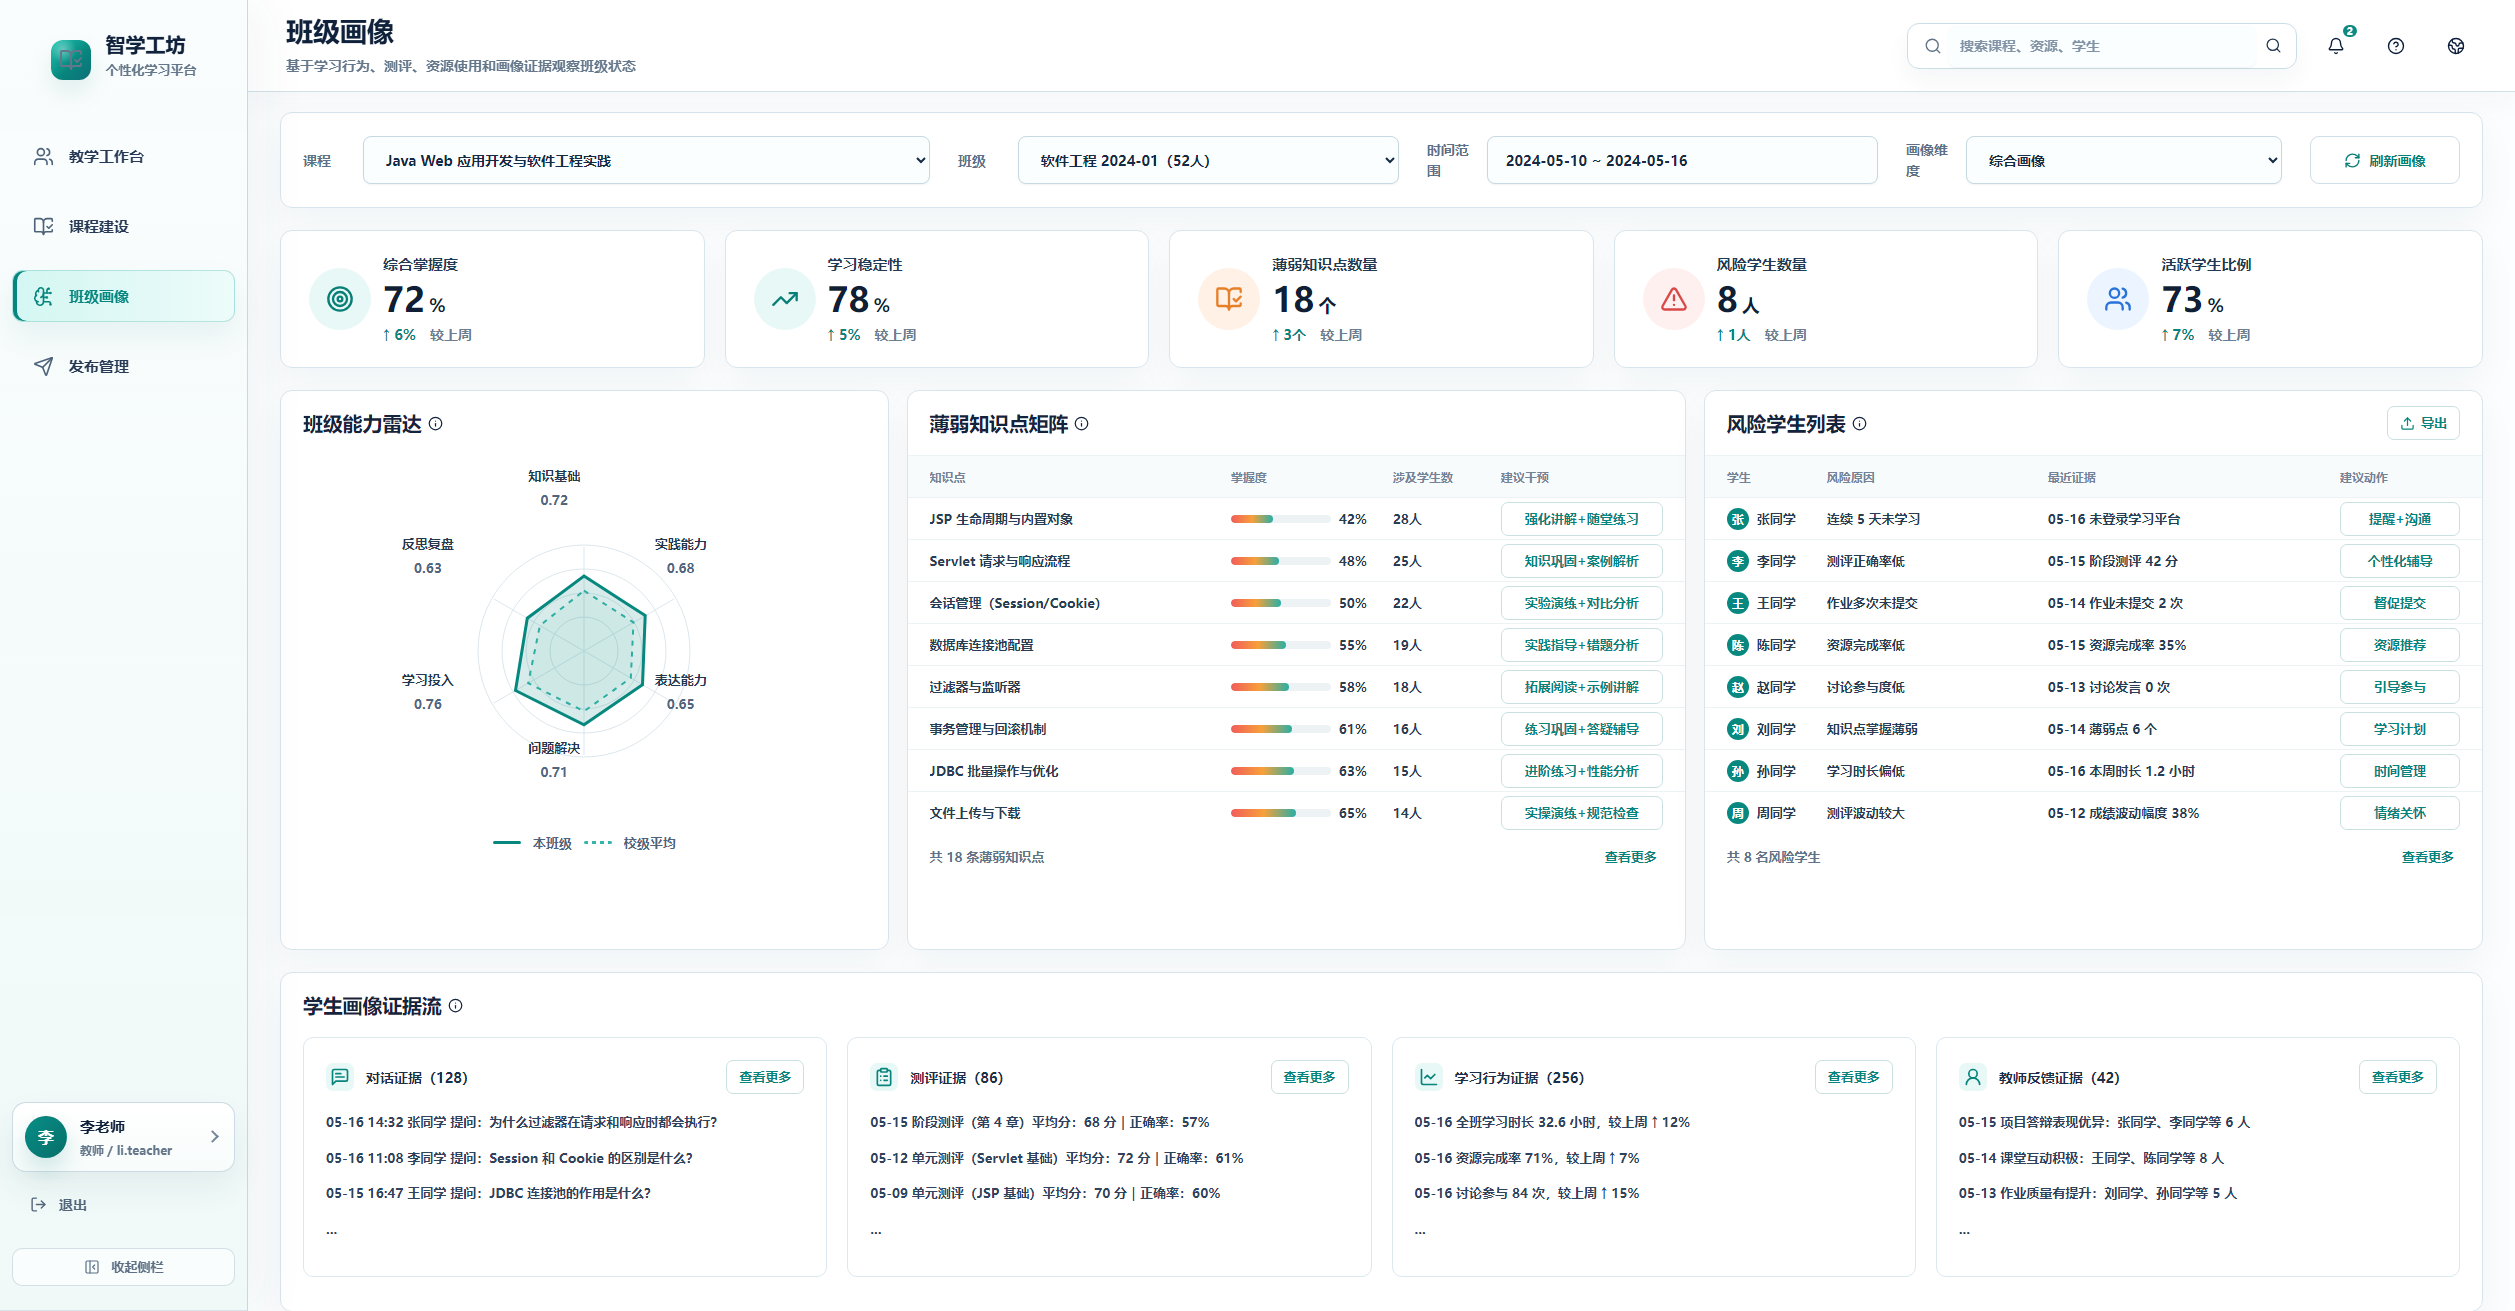
\includegraphics[width=0.92\textwidth]{teacher-class-profile-approved.png}
\end{figure}
\end{frame}

\begin{frame}{教师端：资源审核与质量门禁}
\begin{figure}
\centering
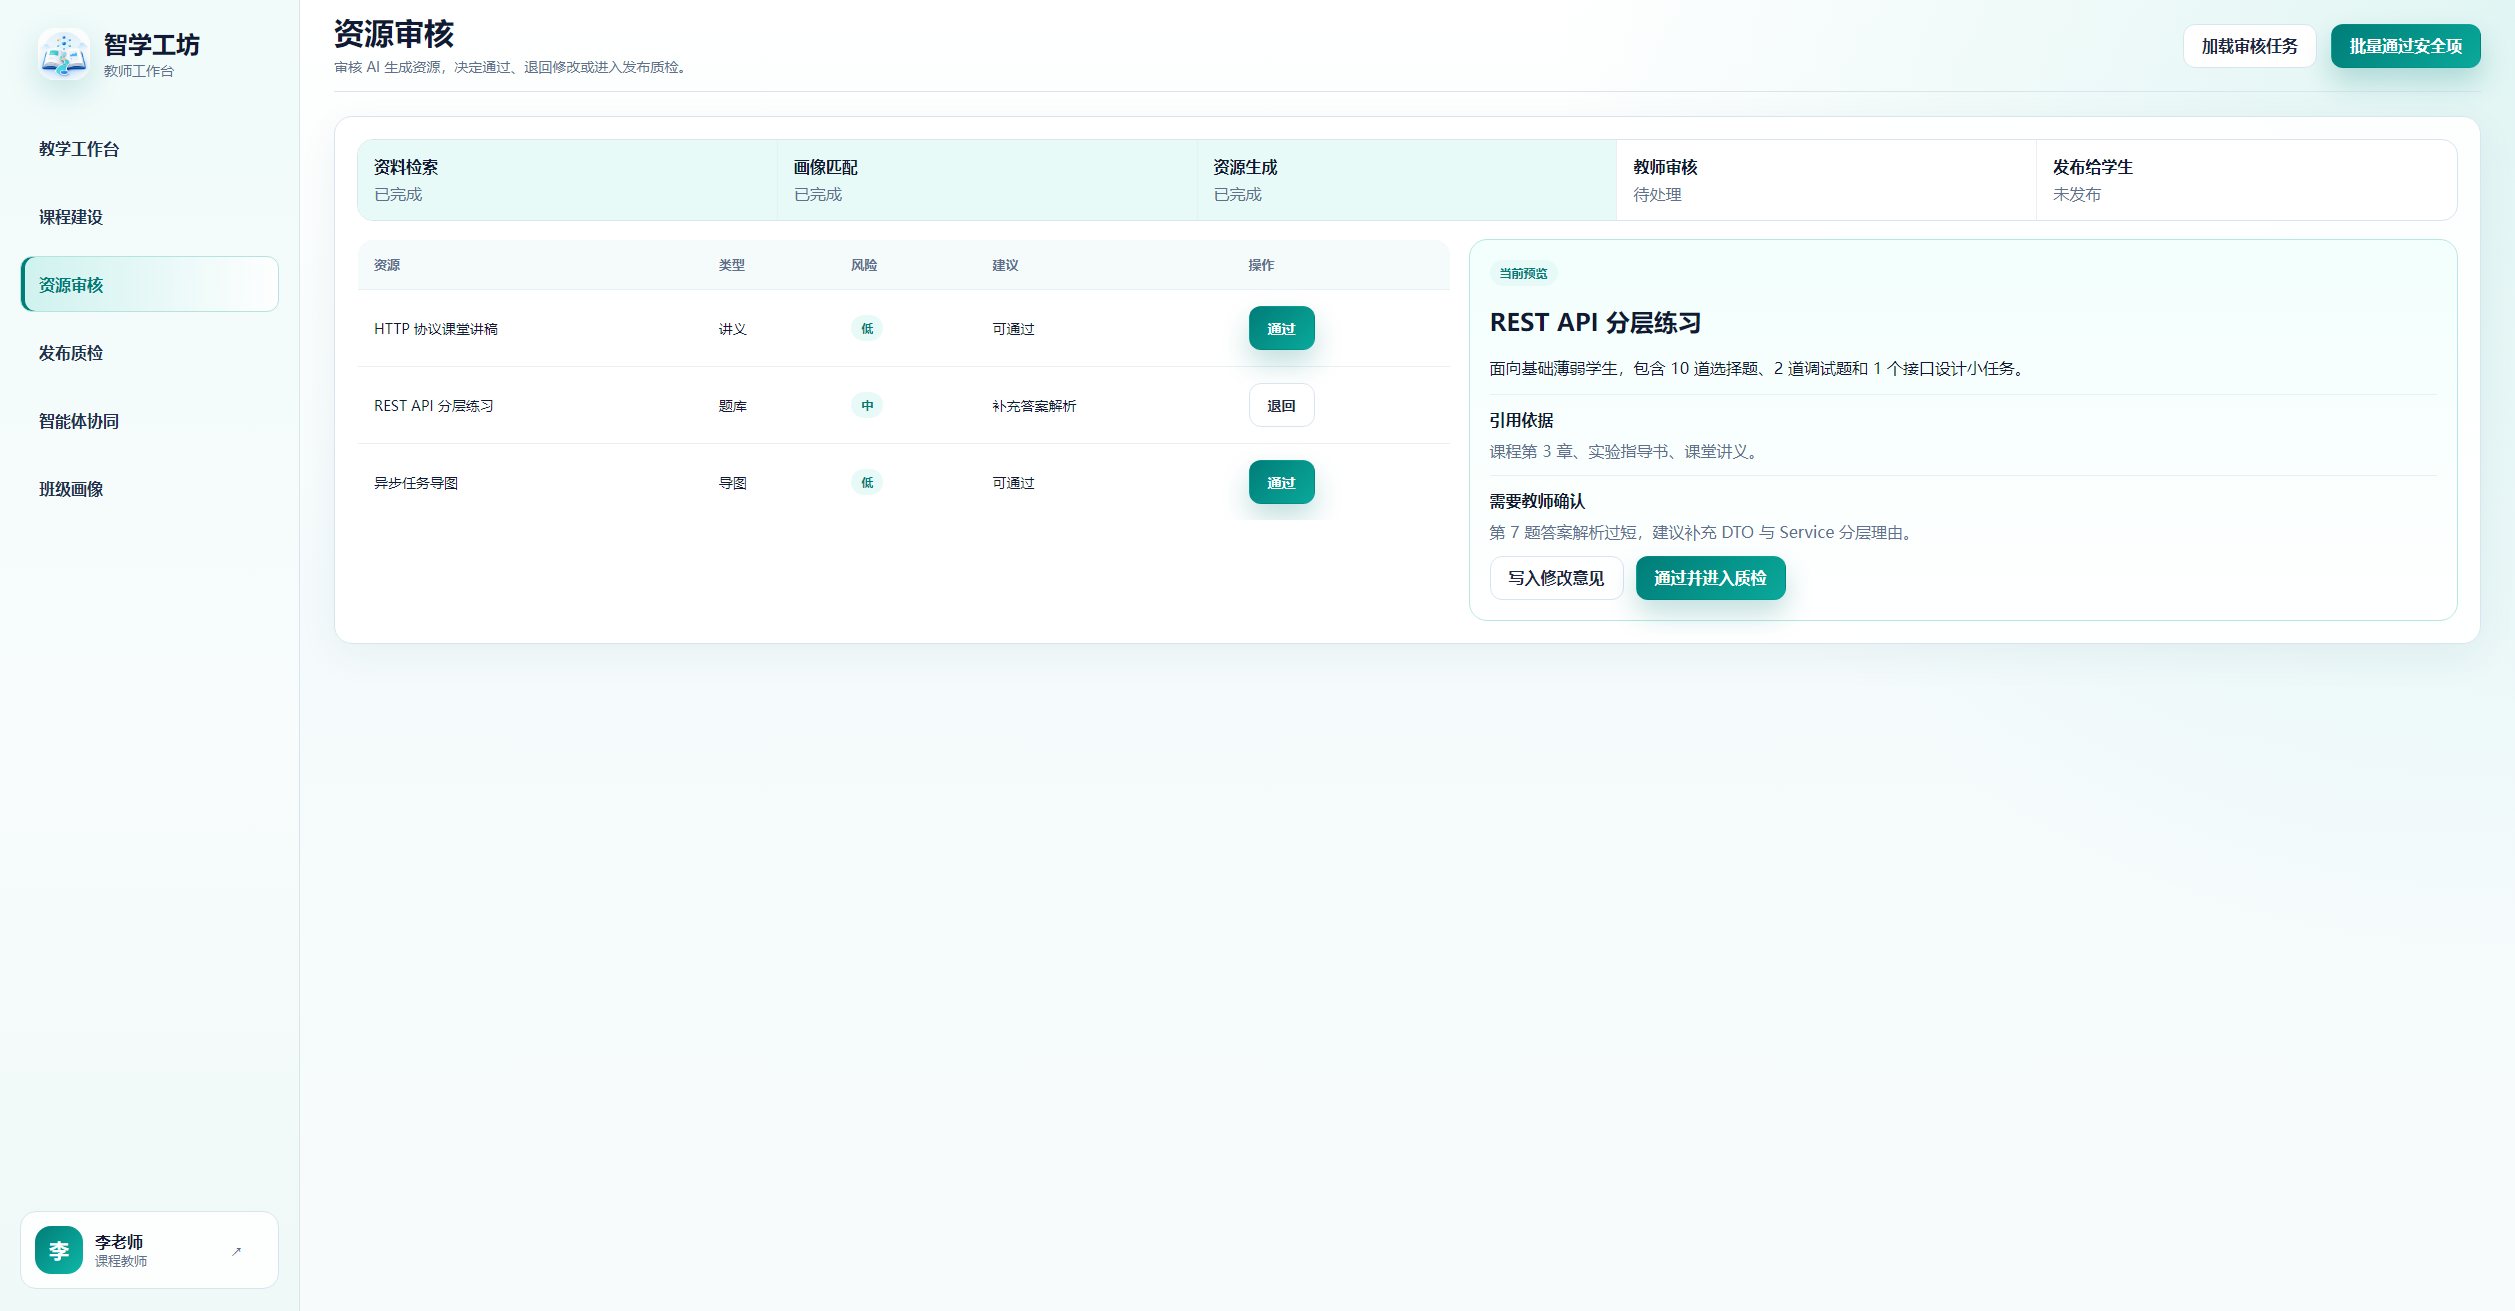
\includegraphics[width=0.92\textwidth]{04-teacher-resource-review-v1.png}
\end{figure}
\end{frame}

\section{技术实现}

\begin{frame}{讯飞星火接入}
\begin{itemize}
  \item 正式模型提供方：科大讯飞星火 API。
  \item 密钥通过环境变量注入：\texttt{XFYUN\_API\_PASSWORD} 或 \texttt{XFYUN\_API\_KEY/XFYUN\_API\_SECRET}。
  \item 支持调用缓存与每日调用限额，适配比赛演示额度较少的情况。
  \item 模型调用记录可追踪：模型、端点、提示哈希、缓存命中和错误信息。
\end{itemize}
\end{frame}

\begin{frame}{防幻觉与内容安全}
\begin{table}
\centering
\begin{tabular}{p{0.28\textwidth} p{0.58\textwidth}}
\toprule
\textbf{风险} & \textbf{控制措施} \\
\midrule
无依据生成 & RAG 检索课程资料，输出引用覆盖情况 \\
事实性错误 & 审计智能体检查断言和证据匹配 \\
敏感内容 & 发布前进行内容安全过滤和人工复核门禁 \\
降级/兜底 & 后端校验 fallbackUsed，拒绝任何降级结果入库 \\
长任务等待 & 任务步骤、事件流和进度状态可视化 \\
额度消耗 & 启用缓存、每日限额和演示脚本预热 \\
\bottomrule
\end{tabular}
\end{table}
\end{frame}

\begin{frame}{满足赛题功能要求}
\begin{itemize}
  \item 对话式画像：8 个维度（超出赛题 6 维要求），随学习事件动态更新。
  \item 多智能体资源生成：覆盖 7 类资源（超出赛题 5 类要求），保留阶段与证据。
  \item 学习路径规划：结合课程进度、画像短板和任务截止时间，章节精准推送。
  \item 智能辅导：RAG 课程上下文问答 + Mermaid 图解 + 资料引用 + 疑惑沉淀。
  \item 学习效果评估：课程作业测试自动评分、跨课程画像、证据流和干预建议。
\end{itemize}
\end{frame}

\begin{frame}{现代 AI 交互与多模态}
\begin{itemize}
  \item 流式 Markdown 输出，答疑结果实时渲染。
  \item Mermaid 图解渲染：思维导图、答疑图解以真实图形多模态呈现。
  \item 生成进度追踪：进度条、当前步骤、百分比实时刷新，避免白屏等待。
  \item 课程任务：作业/测试在课程内完成，测试自动评分、提交持久化。
  \item 多模型热切换：讯飞星火与 DeepSeek / 通义 / 智谱等供应商运行时可切换。
\end{itemize}
\end{frame}

\begin{frame}{创新亮点}
\begin{enumerate}
  \item 课程为中心的 AI 项目空间，而非孤立的资源任务入口。
  \item 真正的多智能体协同：LangGraph 编排，链路全程可追踪。
  \item 可信 AI 工程闭环：RAG 限定 + 审计智能体 + 后端拒绝降级结果。
  \item 双端协同：学生学习闭环 + 教师 AI 建课、课程诊断、发布质量门禁。
  \item 学习数据回流：事件、测评、疑惑文档持续反哺画像与推送策略。
\end{enumerate}
\end{frame}

\section{交付与演示}

\begin{frame}{交付物}
\begin{itemize}
  \item 作品安装包或可执行文件：后端 jar、前端静态文件、Python 智能体、启动脚本。
  \item 作品源码：前端、后端、智能体、数据库迁移、课程数据和文档。
  \item PPT/文档：基于 Beamer-HFUT 的演示文稿、设计说明、使用说明、测试说明、AI Coding 说明。
  \item 演示视频脚本：7 分钟内展示学生学习闭环、教师审核发布和多智能体生成链路。
\end{itemize}
\end{frame}

\begin{frame}{演示路线}
\begin{enumerate}
  \item 学生登录，查看今日学习计划。
  \item 进入我的课程，打开课程详情页。
  \item 在课程 AI 助手中提问并生成个性化资源。
  \item 查看任务进度、生成记录和学习画像。
  \item 教师登录，审核资源并进行发布质检。
  \item 总结讯飞星火、多智能体、防幻觉和学习闭环。
\end{enumerate}
\end{frame}

\begin{frame}{总结}
\begin{block}{智学工坊}
以课程为中心，把讯飞大模型、多智能体资源生成、学习画像和教师审核发布串成可运行、可追踪、可持续迭代的个性化学习平台。
\end{block}
\vspace{0.8cm}
\begin{center}
谢谢各位！
\end{center}
\end{frame}

\end{document}
